\section{OBSERVED-EXPOSURE REMOVAL SENSITIVITY}
\label{app:dose}
This exploratory follow-up was specified after external feedback on the manuscript. The Amazon/Tolokers grid was fixed before its outcomes were inspected; the Weibo extension was specified after those two-graph results, before fitting its supervised models. We retain both scorers and every condition. Weibo uses the official file described in Appendix~\ref{app:fresh}, the same fixed classifier settings as Appendix~\ref{app:supervised}, and a uniform 10\% training panel (840 labels), with ten training seeds and five test splits per seed. Its graph features use the same unweighted neighbor means and log degree. Training runs use one CPU thread; no Weibo outcome was used to tune model settings.

\begin{table}[ht]\centering\small
\caption{Ranking quality on all nontraining nodes: mean $\pm$ SD across ten training seeds. Average precision is reported alongside AUROC because discovery uses the upper score tail.}
\begin{tabular}{llrr}\toprule Graph & Score & AUROC & Average precision\\\midrule
Amazon & Attributes & $0.969\pm0.002$ & $0.895\pm0.007$ \\
Amazon & Attributes + graph & $0.971\pm0.005$ & $0.898\pm0.009$ \\
Tolokers & Attributes & $0.706\pm0.009$ & $0.345\pm0.012$ \\
Tolokers & Attributes + graph & $0.790\pm0.006$ & $0.472\pm0.011$ \\
Weibo & Attributes & $0.929\pm0.006$ & $0.292\pm0.014$ \\
Weibo & Attributes + graph & $0.948\pm0.003$ & $0.338\pm0.015$ \\
\bottomrule\end{tabular}\end{table}

For each test split, independently reveal each non-test deployment label with probability $\rho\in\{0.25,0.50,1\}$, using nested draws. Exposure is the number of neighbors known anomalous from training or revealed non-test labels, divided by graph degree (zero for isolated nodes). Only revealed normal deployment nodes are eligible calibration nodes. At removal fraction $d$, retain $\lceil(1-d)M\rceil$ of these $M$ nodes. The exposure rule retains the smallest exposures, using a fresh uniform tie ordering each repetition; the comparator retains a uniform subset of identical size. Both orderings are shared across scorers and removal fractions within a repetition. Independent node-level uniform marks resolve score ties lexicographically once per scorer before the evaluation splits; they never reverse a strict score order.

The nine removal fractions are $0,.05,.10,.20,.40,.60,.80,.90,.97$. Each graph--scorer--seed--split--revelation--fraction--rule has 50 repetitions, giving 810,000 evaluations across three graphs. Repetitions and splits are averaged within training seed before computing the reported means and seed SDs. At zero removal the two rules are identical. Unlike the original zero-exposure comparison, no fixed 1,000-node cap restricts the remaining reference. The 100\% revelation condition still excludes every test label and is not the oracle zero-exposure intervention.

All 450 graph--seed--split--revelation checks leave exposure unchanged when every unknown label is flipped. Disjointness, normal-only references, matched sample sizes, and identical zero-removal outcomes are asserted in the run. One hundred random tied-score examples check the optimized score-ordered BH implementation against the independent reference implementation after applying the same tie convention. Saved protocols, scores, complete compressed trials, split summaries, seed summaries, and hashes support reproduction without GPU training. Figures~\ref{fig:doseallfdp} and~\ref{fig:doseallpower} report the full grid. The tables below isolate the prespecified mild-removal fractions; remaining numerical cells, including their SDs and discovery counts, are in the complete summary CSV.
\begin{table}[ht]\centering\small
\caption{Amazon: all mild-removal outcomes, mean FDP / power. Each pair uses the same remaining reference size; $\rho$ is the revealed non-test label fraction.}
\begin{tabular}{llrrr}\toprule Score & $\rho$ & Removed & Exposure & Random\\\midrule
Attributes & 0.25 & 0.05 & $0.095/0.782$ & $0.090/0.777$ \\
Attributes & 0.25 & 0.10 & $0.105/0.791$ & $0.089/0.775$ \\
Attributes & 0.25 & 0.20 & $0.111/0.793$ & $0.088/0.773$ \\
Attributes & 0.50 & 0.05 & $0.096/0.785$ & $0.089/0.779$ \\
Attributes & 0.50 & 0.10 & $0.107/0.793$ & $0.088/0.779$ \\
Attributes & 0.50 & 0.20 & $0.119/0.799$ & $0.088/0.778$ \\
Attributes & 1.00 & 0.05 & $0.097/0.788$ & $0.091/0.783$ \\
Attributes & 1.00 & 0.10 & $0.113/0.796$ & $0.091/0.782$ \\
Attributes & 1.00 & 0.20 & $0.124/0.804$ & $0.091/0.782$ \\
Attributes + graph & 0.25 & 0.05 & $0.095/0.789$ & $0.088/0.776$ \\
Attributes + graph & 0.25 & 0.10 & $0.109/0.801$ & $0.087/0.773$ \\
Attributes + graph & 0.25 & 0.20 & $0.134/0.815$ & $0.087/0.772$ \\
Attributes + graph & 0.50 & 0.05 & $0.103/0.798$ & $0.092/0.789$ \\
Attributes + graph & 0.50 & 0.10 & $0.118/0.807$ & $0.091/0.789$ \\
Attributes + graph & 0.50 & 0.20 & $0.145/0.820$ & $0.091/0.788$ \\
Attributes + graph & 1.00 & 0.05 & $0.102/0.798$ & $0.091/0.792$ \\
Attributes + graph & 1.00 & 0.10 & $0.123/0.811$ & $0.091/0.792$ \\
Attributes + graph & 1.00 & 0.20 & $0.153/0.825$ & $0.091/0.791$ \\
\bottomrule\end{tabular}\end{table}
\begin{table}[ht]\centering\small
\caption{Tolokers: all mild-removal outcomes, mean FDP / power. Each pair uses the same remaining reference size; $\rho$ is the revealed non-test label fraction.}
\begin{tabular}{llrrr}\toprule Score & $\rho$ & Removed & Exposure & Random\\\midrule
Attributes & 0.25 & 0.05 & $0.000/0.000$ & $0.000/0.000$ \\
Attributes & 0.25 & 0.10 & $0.009/0.000$ & $0.000/0.000$ \\
Attributes & 0.25 & 0.20 & $0.000/0.000$ & $0.001/0.000$ \\
Attributes & 0.50 & 0.05 & $0.000/0.000$ & $0.000/0.000$ \\
Attributes & 0.50 & 0.10 & $0.000/0.000$ & $0.001/0.000$ \\
Attributes & 0.50 & 0.20 & $0.000/0.000$ & $0.001/0.000$ \\
Attributes & 1.00 & 0.05 & $0.000/0.000$ & $0.000/0.000$ \\
Attributes & 1.00 & 0.10 & $0.000/0.000$ & $0.000/0.000$ \\
Attributes & 1.00 & 0.20 & $0.000/0.000$ & $0.001/0.000$ \\
Attributes + graph & 0.25 & 0.05 & $0.006/0.001$ & $0.008/0.001$ \\
Attributes + graph & 0.25 & 0.10 & $0.006/0.001$ & $0.009/0.001$ \\
Attributes + graph & 0.25 & 0.20 & $0.006/0.001$ & $0.010/0.001$ \\
Attributes + graph & 0.50 & 0.05 & $0.021/0.001$ & $0.022/0.001$ \\
Attributes + graph & 0.50 & 0.10 & $0.023/0.001$ & $0.023/0.001$ \\
Attributes + graph & 0.50 & 0.20 & $0.031/0.001$ & $0.027/0.001$ \\
Attributes + graph & 1.00 & 0.05 & $0.045/0.001$ & $0.030/0.001$ \\
Attributes + graph & 1.00 & 0.10 & $0.050/0.001$ & $0.032/0.001$ \\
Attributes + graph & 1.00 & 0.20 & $0.051/0.002$ & $0.029/0.001$ \\
\bottomrule\end{tabular}\end{table}
\begin{table}[ht]\centering\small
\caption{Weibo: all mild-removal outcomes, mean FDP / power. Each pair uses the same remaining reference size; $\rho$ is the revealed non-test label fraction.}
\begin{tabular}{llrrr}\toprule Score & $\rho$ & Removed & Exposure & Random\\\midrule
Attributes & 0.25 & 0.05 & $0.283/0.069$ & $0.000/0.000$ \\
Attributes & 0.25 & 0.10 & $0.577/0.255$ & $0.001/0.000$ \\
Attributes & 0.25 & 0.20 & $0.583/0.256$ & $0.003/0.000$ \\
Attributes & 0.50 & 0.05 & $0.424/0.069$ & $0.013/0.001$ \\
Attributes & 0.50 & 0.10 & $0.657/0.332$ & $0.013/0.001$ \\
Attributes & 0.50 & 0.20 & $0.655/0.338$ & $0.013/0.001$ \\
Attributes & 1.00 & 0.05 & $0.458/0.075$ & $0.019/0.000$ \\
Attributes & 1.00 & 0.10 & $0.668/0.352$ & $0.019/0.000$ \\
Attributes & 1.00 & 0.20 & $0.674/0.376$ & $0.006/0.000$ \\
Attributes + graph & 0.25 & 0.05 & $0.341/0.109$ & $0.000/0.000$ \\
Attributes + graph & 0.25 & 0.10 & $0.665/0.647$ & $0.001/0.000$ \\
Attributes + graph & 0.25 & 0.20 & $0.666/0.615$ & $0.003/0.000$ \\
Attributes + graph & 0.50 & 0.05 & $0.429/0.128$ & $0.001/0.000$ \\
Attributes + graph & 0.50 & 0.10 & $0.683/0.771$ & $0.003/0.000$ \\
Attributes + graph & 0.50 & 0.20 & $0.683/0.771$ & $0.006/0.000$ \\
Attributes + graph & 1.00 & 0.05 & $0.499/0.143$ & $0.004/0.000$ \\
Attributes + graph & 1.00 & 0.10 & $0.691/0.811$ & $0.008/0.000$ \\
Attributes + graph & 1.00 & 0.20 & $0.696/0.838$ & $0.003/0.000$ \\
\bottomrule\end{tabular}\end{table}
\clearpage\begin{figure}[p]\centering
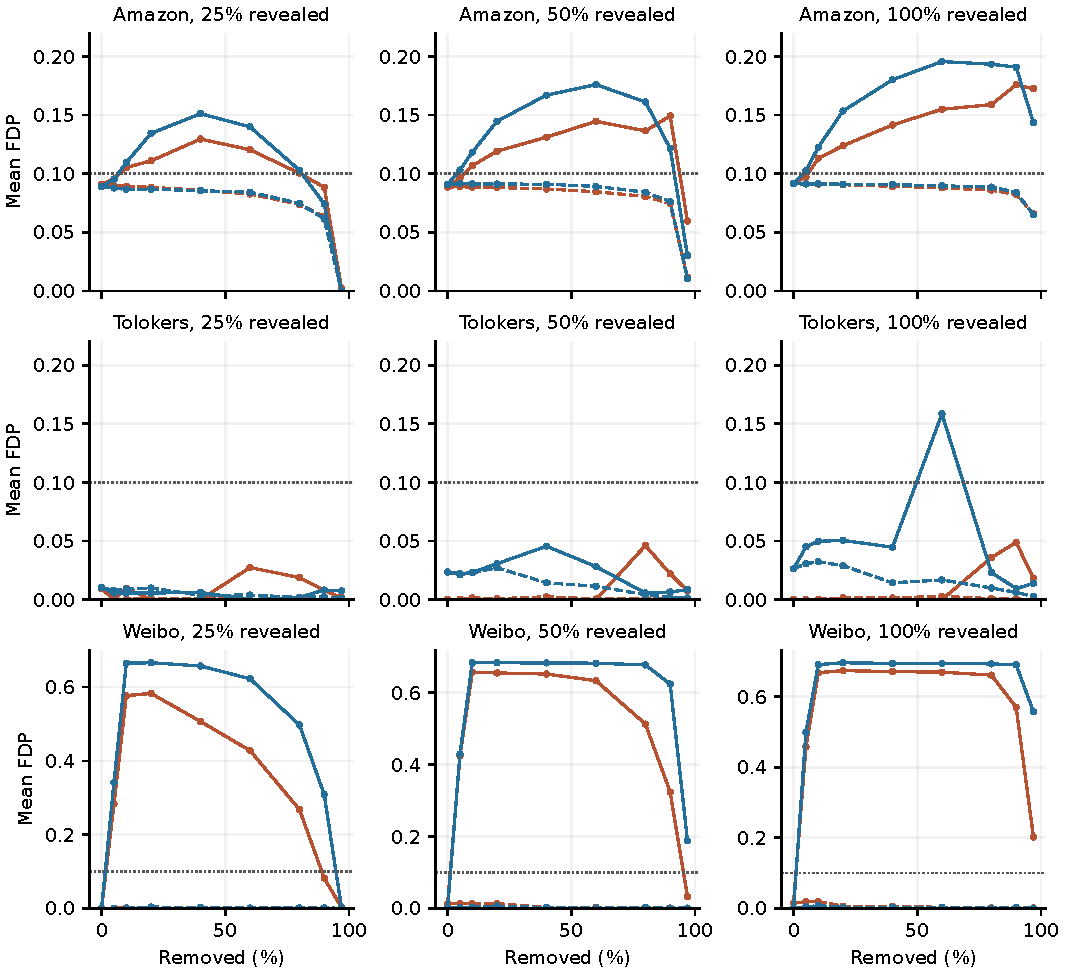
\includegraphics[width=.96\textwidth]{selection_dose_all_fdp.pdf}
\caption{Complete removal grid: mean FDP over training-seed averages, including abstention. Orange is attributes; blue adds graph features. Solid lines remove by observed exposure; dashed lines remove uniformly. Every cell uses ten training seeds, five splits, and 50 paired repetitions. Different graphs may have different vertical scales.}
\label{fig:doseallfdp}\end{figure}
\clearpage\begin{figure}[p]\centering
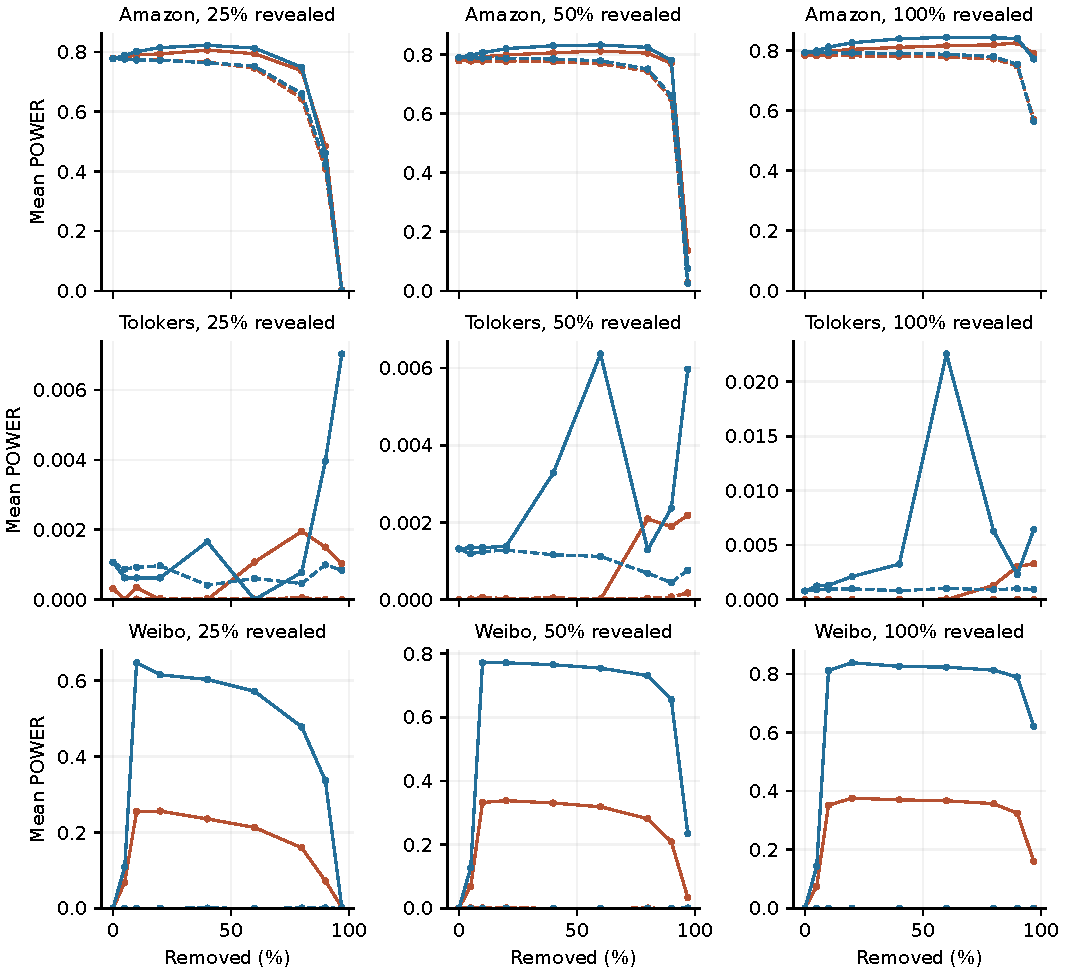
\includegraphics[width=.96\textwidth]{selection_dose_all_power.pdf}
\caption{Complete removal grid: mean POWER over training-seed averages, including abstention. Orange is attributes; blue adds graph features. Solid lines remove by observed exposure; dashed lines remove uniformly. Every cell uses ten training seeds, five splits, and 50 paired repetitions. Different graphs may have different vertical scales.}
\label{fig:doseallpower}\end{figure}
